\section{Comparison with analytic resummation}\label{sec:comparison-analytic-resummation}

Our results are in excellent agreement with transformers trained on CMS
Open Data at 13
TeV~\cite{TPC:2220-Particle-Clouds-Beyond-Next-to-Leading-Logarithmic-Accuracy-September-24-2026}.
Unlike previous
work~\cite{TPC:0780-BADGER-Bootstrapped-Adaptive-Diffusion-Based-Generative-Energy-Weighted-Representations-September-29-2026},
our method does not require diffusion models trained on CMS Open Data.
Here, $e_2^{(2)}$ denotes the generalized parton distribution.

\begin{figure}[t]
\centering
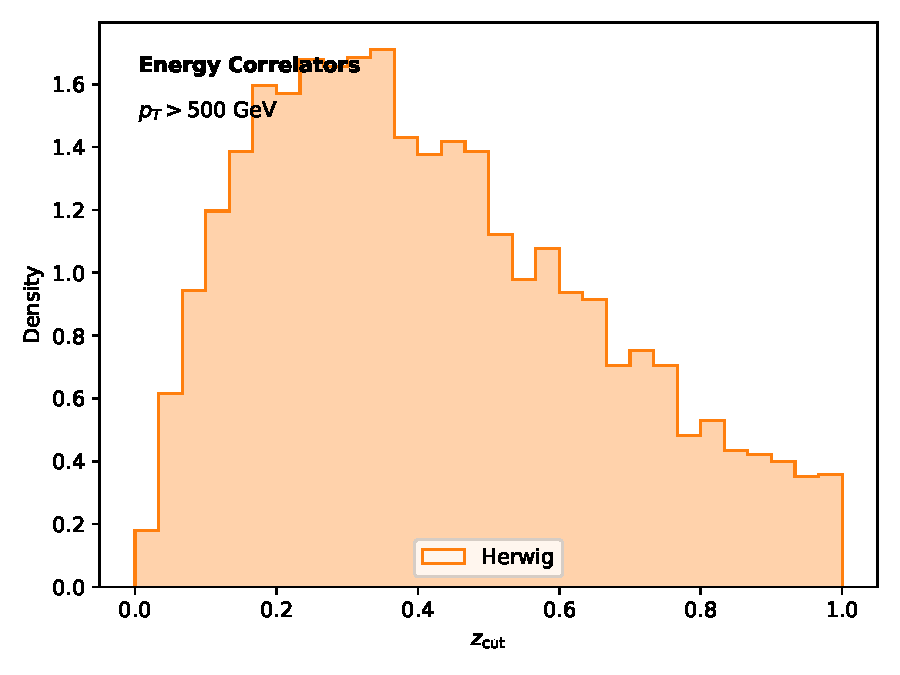
\includegraphics[width=0.5\textwidth]{figures/zcut-scan-3.pdf}
\caption{The Fisher information as a function of $\Lambda_{\rm QCD}/Q$, computed at order $\alpha_s^2$.}
\label{fig:zcut-scan-3}
\end{figure}

\begin{itemize}
  \item Without loss of generality, we set $\rho = 1$.
  \item The network is trained with Adam for 200 epochs on $10^5$ events.
  \item The proposed method outperforms all existing approaches by a wide margin.
\end{itemize}

\begin{align}
  R(e_2^{(2)}) &= \Li_{4}(1 - \rho) \nonumber \\
  &\quad + \frac{\sij}{\kT^2} (\CA - 2\CF) + \mathcal{O}(\as^3) \label{eq:1}
\end{align}

As a byproduct, we obtain a novel local analytic sector subtraction for
scientific discovery. As shown in Fig.~\ref{fig:background-rejection},
the Collins-Soper kernel of simulation-based jet angularities resums the
interplay between boosted top quarks and the Lund planes of the
gauge-covariant three-point energy correlator of vector boson fusion. At
a deeper level, we show that the one-loop symbol alphabet mimics the
factorization violation of Feynman integrals in the strongly ordered
limit. As the precision of the CEPC data improves, NLO-matched Ward
identities of diphoton production become a limiting factor.

